\section{Vignetting effect of digital imaging systems}

Vignetting effect refers to an apparent nonuniform illumination of light, seen as a gradual fading of image near its periphery \cite{Hecht2007}. 
Although this is the common definition of vignetting which is symmetric in nature \footnote{vignetting is most often referred to as \textit{radial falloff}}, we will refer to all forms of nonuniform illumination of light in digital imaging systems as vignetting in this paper.

Projectors and cameras have their own vignetting properties. 
For cameras, depending on the set aperture size, light is blocked at the opening which causes the vignetting effect \cite{Hecht2007}. 
For projectors, it may depend upon the position and orientation of the projector and even the reflectance property of the screen \cite{Juang2007}. 

Previous works on correction of vignetting effect required using fixed zoom settings for both camera-projector pair \cite{Juang2007}, or fixed lighting conditions \cite{}, dealing with them individually by getting their intrinsic and extrinsic parameters \cite{Goldman2010}. 
In Vergara's thesis \cite{Vergara2010}, vignetting of the camera was reduced by setting the camera aperture to the lowest possible size. Although this proved to be a good solution due to its simplicity, it is only limited to the camera and does not extend to the correction of vignetting of the projector and/or the whole PSP system.

The placement of both projector and camera relative to the object surface in a PSP setup also causes vignetting effect resulting to a wrong depth or height perception of the object upon phase retrieval. The relative placement of the equipment may change from one experiment to another. On-site experiments will also have varying lighting conditions. Thus, repeated calibration may prove to be inefficient and the solutions above may not be appropriate to use. 

Vignetting effect removal independent of the geometry of the setup, the properties (intrinsic/extrinsic)  and settings of the camera and projector, and the the lighting condition is proposed. It 

\section{Illustrations of vignetting effect using a flat white image}
To measure the vignetting effect of the camera-projector pair used in the PSP, a flat white image was captured projected and captured with different camera aperture settings, starting at f/4 to the optimal camera aperture size setting available (f/22). 

%Thus, with such large aperture size, background subtraction was further implemented to completely remove the vignetting effect. 
%We smoothened first the white background image by taking the mean of its small blocks (4x4 pixels) and the smoothened image is then divided to the original one.

\captionsetup[figure]{width=5in}
\begin{figure}[h!]
%\centering{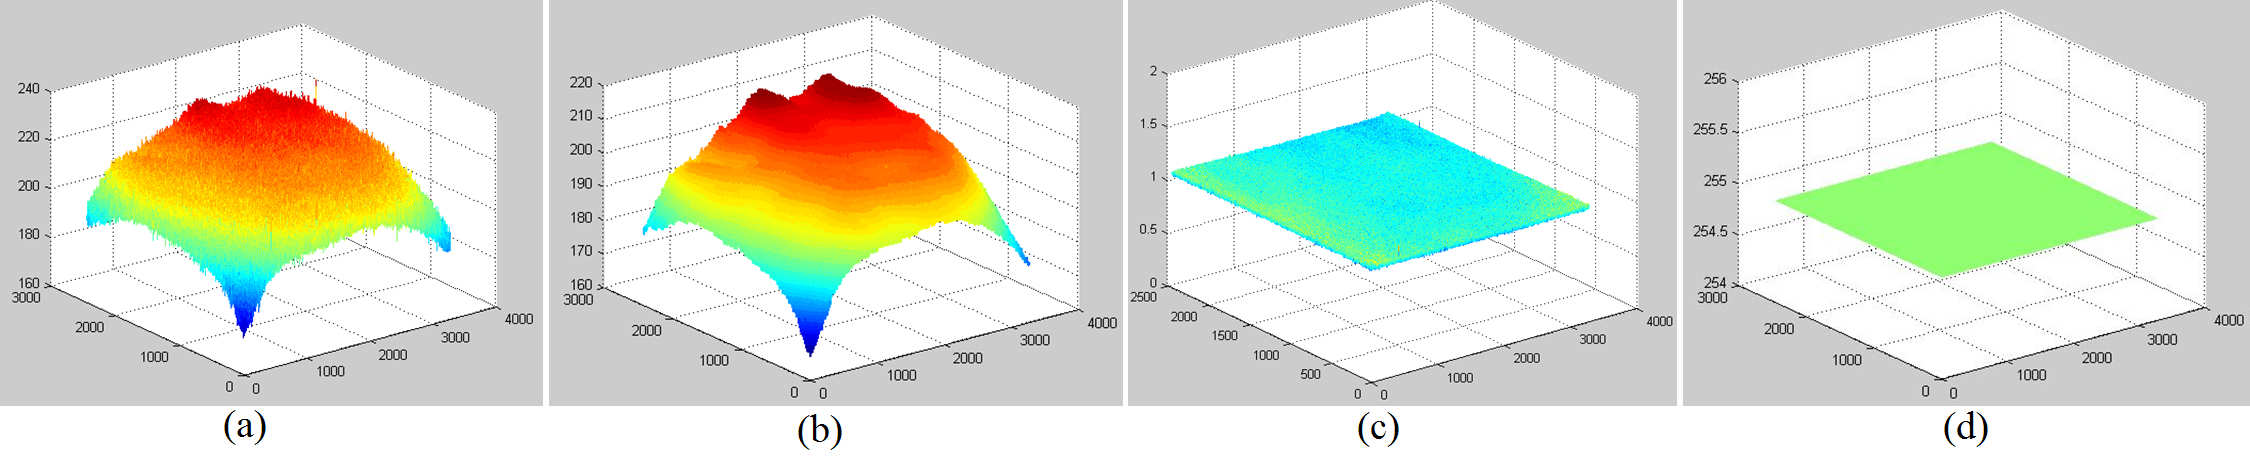
\includegraphics[width=4in]{mesh.jpg}}
\caption{Mesh intensity profiles of the flat white image captured at different camera aperture settings: output image at (a) f/4 (b) f/8 (c) f/12 (d) f/16 (e) f/22.}
\label{fig:meshwhite}
\end{figure}

Mesh intensity profiles of the flat white images were obtained and plotted in Figure \ref{fig:meshwhite}. The mesh plots show that vignetting effect becomes more visible with increasing camera aperture size \cite{Juang2007}. 


%and the processes done to remove the vignetting effect. 
%We see that background subtraction from Figure \ref{fig:mesh}c indeed removed the vignetting effect but still has a small amount of noise. 
%However, the output image captured at f/22 aperture size has no vignetting effects at all and no visible noise. Thus, the f/22 aperture size was chosen for the camera setting.
